\documentclass[11pt,a4paper]{article}

% ------------------------------------------------------------------ packages
\usepackage[T1]{fontenc}
\usepackage[utf8]{inputenc}
\usepackage{lmodern}
\usepackage[scaled=0.92]{helvet}
\usepackage{microtype}
\usepackage[a4paper,margin=2.1cm,top=2.4cm,bottom=2.4cm,headheight=14pt]{geometry}
\usepackage[dvipsnames,table]{xcolor}
\usepackage{graphicx}
\usepackage{booktabs,longtable,tabularx,array,multirow}
\newcolumntype{P}[1]{>{\raggedright\arraybackslash}p{#1}}
\usepackage{enumitem}
\usepackage{fancyhdr}
\usepackage{titlesec}
\usepackage{etoolbox}
\usepackage{lastpage}
\usepackage{fontawesome5}
\usepackage{tikz}
\usepackage[most]{tcolorbox}
\usepackage[hidelinks,bookmarksnumbered]{hyperref}
\usepackage{needspace}
\pretocmd{\section}{\needspace{10\baselineskip}}{}{}
\pretocmd{\subsection}{\needspace{6\baselineskip}}{}{}

% ------------------------------------------------------------------ colours
\definecolor{ink}{HTML}{1F2328}
\definecolor{muted}{HTML}{6E7781}
\definecolor{rule}{HTML}{D0D7DE}
\definecolor{accent}{HTML}{1C5CAB}
\definecolor{accentsoft}{HTML}{E3EEFC}
\definecolor{sevC}{HTML}{C62828}  \definecolor{sevCsoft}{HTML}{FDECEC}
\definecolor{sevM}{HTML}{D9730D}  \definecolor{sevMsoft}{HTML}{FFF3E3}
\definecolor{sevm}{HTML}{8A6D00}  \definecolor{sevmsoft}{HTML}{FFF9DB}
\definecolor{good}{HTML}{1A7F37}  \definecolor{goodsoft}{HTML}{E6F4EA}
\color{ink}

% ------------------------------------------------------------------ typography
\renewcommand{\familydefault}{\sfdefault}
\setlength{\parindent}{0pt}
\setlength{\parskip}{5pt}
\linespread{1.08}
\titleformat{\section}{\Large\bfseries\color{accent}}{\thesection}{0.6em}{}[\vspace{-4pt}{\color{rule}\rule{\linewidth}{0.6pt}}]
\titleformat{\subsection}{\large\bfseries}{\thesubsection}{0.6em}{}
\titlespacing*{\section}{0pt}{16pt}{8pt}
\titlespacing*{\subsection}{0pt}{12pt}{4pt}
\setlist{nosep,leftmargin=1.3em,topsep=2pt}

\pagestyle{fancy}
\fancyhf{}
\fancyhead[L]{\small\color{muted}I-ITSM \textbullet\ Independent audit report}
\fancyhead[R]{\small\color{muted}Commit d1569ab \textbullet\ 15 Nov 2026}
\fancyfoot[C]{\small\color{muted}Page \thepage\ of \pageref{LastPage}}
\renewcommand{\headrulewidth}{0.4pt}
\renewcommand{\headrule}{{\color{rule}\hrule width\headwidth height\headrulewidth}}

% ------------------------------------------------------------------ helpers
\newcommand{\code}[1]{{\ttfamily\small\detokenize{#1}}}
\newcommand{\sevname}[1]{\ifstrequal{#1}{C}{CRITICAL}{\ifstrequal{#1}{M}{MAJOR}{MINOR}}}
\newcommand{\badge}[1]{\tikz[baseline=(b.base)]\node[fill=sev#1,text=white,rounded corners=2pt,inner xsep=4pt,inner ysep=1.5pt,font=\scriptsize\bfseries](b){\sevname{#1}};}
\newcommand{\okbadge}{\tikz[baseline=(b.base)]\node[fill=good,text=white,rounded corners=2pt,inner xsep=4pt,inner ysep=1.5pt,font=\scriptsize\bfseries](b){MET};}
\newcommand{\partbadge}{\tikz[baseline=(b.base)]\node[fill=sevM,text=white,rounded corners=2pt,inner xsep=4pt,inner ysep=1.5pt,font=\scriptsize\bfseries](b){PARTIAL};}
\newcommand{\nobadge}{\tikz[baseline=(b.base)]\node[fill=sevC,text=white,rounded corners=2pt,inner xsep=4pt,inner ysep=1.5pt,font=\scriptsize\bfseries](b){NOT MET};}
\newcommand{\fld}[2]{\textbf{\color{accent}#1.}\ #2\par}
\newcommand{\remark}[1]{{\color{muted}\itshape\faQuoteLeft\ #1}\par}
\newcommand{\iref}[1]{\hyperref[iss:#1]{\textbf{#1}}}
% score bar: \sbar{score}{max}
\newcommand{\sbar}[2]{\begin{tikzpicture}[baseline=-0.6ex]
  \fill[rule] (0,-0.13) rectangle (2.2,0.13);
  \pgfmathsetmacro{\w}{2.2*#1/#2}
  \fill[accent] (0,-0.13) rectangle (\w,0.13);
\end{tikzpicture}}

% issue card: \begin{issue}{ID}{C|M|m}{Title}{Area}{Rubric criterion}
\newenvironment{issue}[5]{%
  \begin{tcolorbox}[enhanced,breakable,colback=white,colframe=rule,boxrule=0.5pt,arc=2pt,
    borderline west={3pt}{0pt}{sev#2},left=8pt,right=6pt,top=4pt,bottom=4pt,
    before skip=8pt,after skip=6pt,
    title={\phantomsection\label{iss:#1}\badge{#2}\hspace{6pt}\textbf{#1}\hspace{6pt}#3},
    coltitle=ink,colbacktitle=sev#2soft,fonttitle=\normalsize,
    detach title,
    before upper={\tcbtitle\par\vspace{2pt}{\small\color{muted}\faFolder[regular]\ #4\quad\faBalanceScale\ #5}\par\vspace{3pt}}]
  \small}{\end{tcolorbox}}

\begin{document}

% ================================================================== TITLE PAGE
\begin{titlepage}
\thispagestyle{empty}
\begin{tikzpicture}[remember picture,overlay]
  \fill[accent] (current page.north west) rectangle ([yshift=-7.2cm]current page.north east);
  \node[anchor=north west,text=white,font=\sffamily] at ([xshift=2.1cm,yshift=-1.6cm]current page.north west)
    {\begin{minipage}{16cm}
      {\large CS F213 / MAC F212 \textbullet\ Object-Oriented Programming \textbullet\ Semester I, 2026--2027}\\[14pt]
      {\fontsize{30}{34}\selectfont\bfseries Independent Audit Report}\\[8pt]
      {\Large I-ITSM: Intelligent IT Service Management \& Incident Resolution System}
     \end{minipage}};
\end{tikzpicture}
\vspace*{6.6cm}

\begin{tabularx}{\textwidth}{@{}>{\color{muted}}l X@{}}
Audited version & GitHub \code{aditya7245/IITSM}, branch \code{main}, commit \code{d1569ab} (15 Nov 2026) \\
Reference & \code{OOP_S1_2026-2027_Project.pdf} (project specification and evaluation rubric) \\
Submission deadline & 22 Nov 2026 (hard deadline, 7 days after this audit) \\
Method & Full static review of backend, frontend and documents; 702 automated tests run; 69 black-box API probes; headless-browser walk-through of all 13 pages on desktop and phone \\
Stance & Deliberately strict. Every issue below was verified against the code or reproduced on the running system.
\end{tabularx}

\vspace{14pt}
\begin{tcolorbox}[colback=accentsoft,colframe=accent,boxrule=0.6pt,arc=3pt,left=10pt,right=10pt,top=8pt,bottom=8pt]
{\large\bfseries Verdict}\par\vspace{4pt}
The software is \textbf{well above average}: all MVP modules work end to end, 702 tests pass, and authorization held up
against every intrusion attempt. It is \textbf{not ready to submit}. The report and video still carry ``Group N'' and
``Member 1--4'' placeholders, the flagship innovation (the AI guide) is missing from every document, a UI bug can
overwrite one user's data with another's, and the ``State pattern'' that the report advertises is a lookup table in
disguise. A strict examiner would mark this at \textbf{about 86 / 120 as it stands}. Fixing the issues marked
\emph{doc} and \emph{quick} in Section~\ref{sec:plan} lifts that to about 105 / 120 within the deadline.
\end{tcolorbox}

\vspace{10pt}
\begin{center}
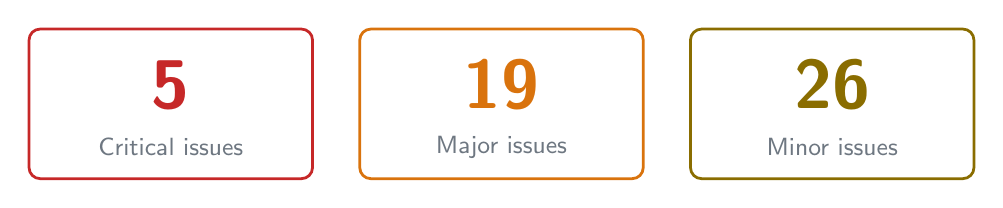
\begin{tikzpicture}
  \foreach \x/\n/\c/\l in {0/5/sevC/Critical, 4.2/19/sevM/Major, 8.4/26/sevm/Minor}{
    \node[draw=\c,line width=1pt,rounded corners=4pt,minimum width=3.6cm,minimum height=1.9cm] at (\x,0) {};
    \node[font=\fontsize{26}{28}\selectfont\bfseries,text=\c] at (\x,0.25) {\n};
    \node[font=\small,text=muted] at (\x,-0.55) {\l\ issues};
  }
\end{tikzpicture}
\end{center}
\vfill
{\small\color{muted}Prepared with Claude Code (Anthropic) as an independent pre-submission review. The marks are an
estimate of how a strict evaluator could score the work; the real evaluation rests with the course instructors.}
\end{titlepage}

% ================================================================== CONTENTS
\tableofcontents
\vspace{8pt}
{\small\color{muted}The full issue index with page numbers is in Section~\ref{sec:index}. Every issue ID in this document is a link.}
\newpage

% ================================================================== 1
\section{Executive summary}

\subsection{What an examiner will see in the first ten minutes}
\begin{enumerate}[leftmargin=1.6em]
\item \textbf{The title page says ``Group N'' and lists ``Member 1--4, ID-1--ID-4''.} The same placeholders appear in
  every page header, in the contributions table and in the video file name (\iref{C-01}, \iref{C-02}).
\item \textbf{The video is narrated by a synthetic voice reading placeholder names.} The rubric requires every member
  to introduce themselves and explain a module (\iref{C-02}).
\item \textbf{The README says the diagrams and report are ``not started''}, although both exist (\iref{M-13}).
\item \textbf{The AI guide, the most ``modern technology'' in the project, appears nowhere in the report}, the diagrams,
  the API appendix or the demo script (\iref{M-10}).
\item \textbf{Report numbers are stale}: 676 tests (actually 702), 10 controllers (11), 12 custom exceptions (13),
  13 repositories (14) (\iref{M-11}).
\end{enumerate}

\subsection{What a careful examiner will find on closer inspection}
\begin{enumerate}[leftmargin=1.6em]
\item Editing one user, then another, saves the first user's data onto the second (\iref{C-03}; reproduced).
\item The State pattern is a transition table with State-pattern class names; all behaviour lives in \code{Incident}
  (\iref{C-04}). The report's claim that ``a new status needs one new class'' is false.
\item Concurrent incident reports push technicians past their workload limit; the UI showed ``8 / 5''
  (\iref{M-01}; reproduced).
\item An employee reporting an incident receives the titles of other employees' incidents that they are forbidden
  to open (\iref{M-03}; reproduced).
\item The spec's own duplicate example (``Payment application unavailable'', ``Payment transaction failing'',
  ``Unable to make payment'') is \emph{not} detected (\iref{M-04}; reproduced).
\item ``Add a notification channel by adding one class'' is false: in-app and e-mail are hard-coded (\iref{M-05}).
\item Anyone with the repository can forge an administrator token whenever the backend runs without
  \code{JWT_SECRET}, which is how the team's own start scripts run it (\iref{M-07}; reproduced).
\end{enumerate}

\subsection{Issue count by area}
\begin{center}
\begin{tabular}{lccc c}
\toprule
\textbf{Area} & \textbf{Critical} & \textbf{Major} & \textbf{Minor} & \textbf{Total}\\
\midrule
Documentation \& presentation & 3 & 5 & 5 & 13\\
OOP design \& patterns        & 1 & 3 & 3 & 7\\
Backend correctness           & 0 & 6 & 9 & 15\\
Security                      & 0 & 3 & 2 & 5\\
Frontend \& UX                & 1 & 2 & 6 & 9\\
Tooling                       & 0 & 0 & 1 & 1\\
\midrule
\textbf{Total} & \textbf{5} & \textbf{19} & \textbf{26} & \textbf{50}\\
\bottomrule
\end{tabular}
\end{center}

% ================================================================== 2
\section{Scope and method}

\subsection{What was audited}
The latest \code{origin/main} (commit \code{d1569ab}): the teammates' commits up to \code{b55d90f} plus the AI-guide
commit. That is 294 backend files, 32 frontend source files, the report (\code{docs/report/report.tex} and the built
\code{report.pdf}, 46 pages), 13 PlantUML diagrams, \code{docs/TEST_CASES.md}, \code{docs/demo-script.md}, the README
and the start/stop scripts. The locally rendered demo video (kept outside Git on purpose) was inspected through its
source script.

\subsection{How}
\begin{description}[leftmargin=0pt,style=nextline]
\item[Automated tests] \code{mvn test} on the exact audited tree: \textbf{702 tests, 0 failures, 0 errors}.
  \code{npm run build} succeeds.
\item[Black-box API probes] 69 scripted checks against the running backend in \code{dev,demo} mode (Appendix~\ref{app:probes}):
  the three spec workflows, invalid transitions, input validation, all 8 search criteria, role checks, access to other users' data, forged and
  tampered tokens, deactivated accounts, CORS, brute force and a concurrency burst. 67 passed. The 2 failures and 3
  warnings became issues.
\item[Browser walk-through] Headless Chrome visited all 13 pages as employee, technician and admin at 1400\,px and
  390\,px: \textbf{no console errors, no failed requests, no horizontal overflow}, and every cross-role URL redirects
  home. Two bugs were reproduced visually (Appendix~\ref{app:shots}).
\item[Static review] Four independent passes: backend correctness and security, OOP design and patterns, frontend and
  UX, documentation against the specification. Each reported finding was then re-checked by hand. Two candidate
  findings turned out to be wrong and were dropped. For example, the effective duplicate threshold is 0.3 (migration V4),
  not the 0.5 seeded in V2.
\end{description}

\subsection{Severity scale}
\begin{tabularx}{\textwidth}{@{}l X@{}}
\badge{C} & A mandatory deliverable or requirement visibly fails, or data gets corrupted. An examiner will notice and deduct heavily.\\[3pt]
\badge{M} & A real defect, a false claim in the documents, or a design flaw that an attentive examiner or a viva question will expose.\\[3pt]
\badge{m} & Robustness, polish or consistency. Small deductions, but they add up and colour the examiner's mood.\\
\end{tabularx}

% ================================================================== 3
\section{Evaluation against the rubric}
\label{sec:rubric}
The rubric table in the specification is laid out ambiguously: the criteria column and the description column are
misaligned. This audit reads it as follows, which is the only reading where the marks add up to 120.

\renewcommand{\arraystretch}{1.35}
\begin{longtable}{@{}P{3.4cm} P{1.1cm} P{3.4cm} P{7.4cm}@{}}
\toprule
\textbf{Criterion} & \textbf{Max} & \textbf{Strict estimate} & \textbf{Why}\\
\midrule
\endhead
System Design \& Architecture (problem understanding, clear prototype) & 10 & \sbar{7}{10}\ \textbf{7} &
Clean layering (controllers never touch entities or repositories), a real Observer, Strategy and Repository. Lost
marks: the pseudo State pattern (\iref{C-04}), class and sequence diagrams that do not match the code (\iref{M-16}).\\
Functionality Implementation (mandatory MVP modules) & 60 & \sbar{48}{60}\ \textbf{48} &
Every MVP module works end to end (Section~\ref{sec:mvp}). Deducted for: data corruption on the edit forms
(\iref{C-03}), workload races (\iref{M-01}), lifecycle dead-ends (\iref{M-06}), the spec's duplicate example failing
(\iref{M-04}), duplicates invisible to staff (\iref{M-17}), a team-lead role with no actions (\iref{M-18}), and no
field-level ``Update'' (\iref{m-13}).\\
User Experience: value-added features (SLA, security, intelligent features) & 10 & \sbar{7}{10}\ \textbf{7} &
Strong SLA handling (pause and resume, warnings, escalation), and authorization held against every probe. Deducted for the
duplicate-title leak (\iref{M-03}), the forgeable token (\iref{M-07}), no rate limits (\iref{M-19}) and an SLA status
that only rises (\iref{M-08}).\\
Technical Depth (code quality, APIs and third parties, scalability) & 15 & \sbar{11}{15}\ \textbf{11} &
Third-party integration (Groq LLM, SMTP), JWT, Flyway, Testcontainers. Deducted for no optimistic locking (\iref{M-02}),
e-mail inside DB transactions (\iref{M-09}), in-memory round-robin state (\iref{m-15}), N+1 queries
(\iref{m-25}) and an anemic domain (\iref{M-15}).\\
Testing \& Validation & 5 & \sbar{4}{5}\ \textbf{4} &
702 tests including real-database integration tests, and 28 documented cases across all six required categories. No
concurrency tests (the race in \iref{M-01} went unseen), no frontend tests, no coverage figure (\iref{m-20}).\\
Innovation (beyond the requirements) & 10 & \sbar{7}{10}\ \textbf{7} &
Automatic escalation, duplicate detection, category suggestion, an analytics dashboard and an AI guide: five items from
the spec's innovation list. The AI guide earns nothing while it is undocumented (\iref{M-10}).\\
Documentation \& Presentation & 10 & \sbar{2}{10}\ \textbf{2} &
The report itself is thorough (all 9 technology questions, 28 test cases, an OOP mapping table). But it carries
placeholders (\iref{C-01}), a placeholder-and-TTS video (\iref{C-02}), stale numbers (\iref{M-11}), no priority
rationale (\iref{M-12}) and a README that contradicts reality (\iref{M-13}).\\
\midrule
\textbf{Total} & \textbf{120} & \sbar{86}{120}\ \textbf{86} & About 72\%. With the documentation fixes alone
(C-01, C-02, M-10 to M-13) the Documentation score could rise to about 8 and Innovation to 9, for about 94. Adding the quick code fixes
in Section~\ref{sec:plan} reaches about 105.\\
\bottomrule
\end{longtable}

% ================================================================== 4
\section{MVP and specification compliance}
\label{sec:mvp}
\begin{longtable}{@{}P{5.2cm} P{1.9cm} P{8.7cm}@{}}
\toprule
\textbf{Requirement (spec)} & \textbf{Status} & \textbf{Evidence}\\
\midrule
\endhead
Three user categories & \okbadge & Employee, Technician (plus Team lead), Administrator (plus IT manager); role guards verified in the browser.\\
Incident create / view / update / assign / resolve / close & \partbadge & All work and were probed live. ``Update'' exists only as status actions and the admin priority override; title, category and impact cannot be corrected (\iref{m-13}).\\
Priority from impact, urgency, criticality & \okbadge & Score $=$ I$\times$U$\times$C with a 100-user bump; the payment outage became P1 in probe W1a. The rationale is undocumented (\iref{M-12}).\\
At least 2 assignment strategies & \okbadge & Skill, load and round-robin, switchable at runtime. Races (\iref{M-01}).\\
SLA calculation, tracking, violation & \okbadge & Deadlines, a pausing clock, AT\_RISK and VIOLATED; escalation reached level 3 in probe W3c. Single-status weakness (\iref{M-08}).\\
At least 2 notification mechanisms & \okbadge & In-app and e-mail (Mailpit). Extensibility claim false (\iref{M-05}).\\
Complete incident history & \partbadge & Lifecycle events are audited (W2j). Notes and admin configuration changes are not (\iref{m-06}).\\
At least 5 search/filter criteria & \okbadge & All 8 of the spec's criteria, including a date range, in both the backend and the admin UI (probes F1).\\
At least 2 intelligent features & \okbadge & Category suggestion, smart assignment, duplicate detection, auto-escalation, SLA risk. The duplicate detector misses the spec example (\iref{M-04}).\\
Persistence & \okbadge & PostgreSQL 16 with Flyway; the audit table is append-only through a trigger.\\
Employee: register, report, track, respond, feedback & \okbadge & Verified end to end (W2a--W2i).\\
Technician: acknowledge, notes, request info, resolve, workload & \okbadge & Verified; the workload tile showed ``8 / 5'' after the race (\iref{M-01}).\\
Admin: users, technicians, services, SLA, categories, strategies, reports, audit & \okbadge & All 10 admin pages load clean on desktop and phone.\\
Prevent inappropriate transitions & \okbadge & NEW$\rightarrow$CLOSED, ASSIGNED$\rightarrow$RESOLVED and others return 409 (S1--S3).\\
At least 2 design patterns & \partbadge & Strategy, Observer, Repository and Factory are genuine; State is nominal (\iref{C-04}).\\
Exception handling for the listed cases & \partbadge & 11 of 12 handled; ``duplicate incident'' has a class that is never thrown (\iref{m-03}).\\
Security: authentication, roles, passwords, validation & \okbadge & BCrypt, JWT, a role on every endpoint; no access to other users' data except the duplicate list (\iref{M-03}).\\
Deliverables 1--9 & \partbadge & All present in some form; team responsibilities and the video fail (\iref{C-01}, \iref{C-02}).\\
At least 15 documented test cases & \okbadge & 28 cases; every referenced test method exists.\\
\bottomrule
\end{longtable}

% ================================================================== 5
\section{Issue index}
\label{sec:index}
{\small
\begin{longtable}{@{}P{1.1cm} P{1.7cm} P{2.8cm} P{8.6cm} r@{}}
\toprule
\textbf{ID} & \textbf{Severity} & \textbf{Area} & \textbf{Issue} & \textbf{Page}\\
\midrule
\endhead
\iref{C-01} & \badge{C} & Documentation & Report full of ``Group N'' / ``Member 1--4'' placeholders; no names or IDs & \pageref{iss:C-01}\\
\iref{C-02} & \badge{C} & Presentation & Video: placeholder names, synthetic voice, members never introduce themselves & \pageref{iss:C-02}\\
\iref{C-03} & \badge{C} & Frontend & Edit forms save one user's data onto another user & \pageref{iss:C-03}\\
\iref{C-04} & \badge{C} & OOP design & ``State pattern'' is a transition table; behaviour lives in \code{Incident} & \pageref{iss:C-04}\\
\iref{C-05} & \badge{C} & Documentation & Report's own claims contradicted by the code it describes & \pageref{iss:C-05}\\
\iref{M-01} & \badge{M} & Backend & Concurrent reports push technicians past their workload limit & \pageref{iss:M-01}\\
\iref{M-02} & \badge{M} & Backend & No optimistic locking: SLA monitor and users overwrite each other & \pageref{iss:M-02}\\
\iref{M-03} & \badge{M} & Security & Duplicate list leaks other employees' incident titles & \pageref{iss:M-03}\\
\iref{M-04} & \badge{M} & Backend & Spec's own duplicate example is not detected & \pageref{iss:M-04}\\
\iref{M-05} & \badge{M} & OOP design & New notification channel cannot be added with one class & \pageref{iss:M-05}\\
\iref{M-06} & \badge{M} & Backend & Lifecycle dead-ends with no admin recovery & \pageref{iss:M-06}\\
\iref{M-07} & \badge{M} & Security & Committed default JWT secret allows forging an admin token & \pageref{iss:M-07}\\
\iref{M-08} & \badge{M} & Backend & One rising SLA status hides resolution warnings and breaches & \pageref{iss:M-08}\\
\iref{M-09} & \badge{M} & Backend & E-mail sent while holding a DB transaction and connection & \pageref{iss:M-09}\\
\iref{M-10} & \badge{M} & Documentation & AI guide missing from report, diagrams, API list, demo & \pageref{iss:M-10}\\
\iref{M-11} & \badge{M} & Documentation & Stale numbers: tests, controllers, exceptions, repositories & \pageref{iss:M-11}\\
\iref{M-12} & \badge{M} & Documentation & Priority algorithm rationale not documented (explicit requirement) & \pageref{iss:M-12}\\
\iref{M-13} & \badge{M} & Documentation & README says diagrams and report ``not started''; written for an AI & \pageref{iss:M-13}\\
\iref{M-14} & \badge{M} & OOP design & Role type code duplicated by the class hierarchy and switched on & \pageref{iss:M-14}\\
\iref{M-15} & \badge{M} & OOP design & Anemic domain: invariants enforced in services, not entities & \pageref{iss:M-15}\\
\iref{M-16} & \badge{M} & Documentation & Class and sequence diagrams show relationships the code lacks & \pageref{iss:M-16}\\
\iref{M-17} & \badge{M} & Frontend & Staff never see duplicate candidates (feature invisible) & \pageref{iss:M-17}\\
\iref{M-18} & \badge{M} & Frontend & Team lead receives escalations but cannot act & \pageref{iss:M-18}\\
\iref{M-19} & \badge{M} & Security & No rate limits: AI-cost and e-mail abuse via open registration & \pageref{iss:M-19}\\
\iref{m-01} & \badge{m} & Backend & Technician can be assigned, resolve and verify their own report & \pageref{iss:m-01}\\
\iref{m-02} & \badge{m} & Backend & Escalation skips unassigned P1s; not reset on reassignment & \pageref{iss:m-02}\\
\iref{m-03} & \badge{m} & OOP design & Dead or unreachable exceptions; hierarchy tied to HTTP & \pageref{iss:m-03}\\
\iref{m-04} & \badge{m} & Backend & Constraint violations reported as ``Database failure'' (503) & \pageref{iss:m-04}\\
\iref{m-05} & \badge{m} & Security & Unbounded text inputs (200 KB description accepted) & \pageref{iss:m-05}\\
\iref{m-06} & \badge{m} & Backend & Audit trail misses notes and all admin configuration changes & \pageref{iss:m-06}\\
\iref{m-07} & \badge{m} & Backend & Date filters and daily chart use UTC; IST users see wrong days & \pageref{iss:m-07}\\
\iref{m-08} & \badge{m} & Frontend & Session expiry hard-reloads and loses work; network blip logs out & \pageref{iss:m-08}\\
\iref{m-09} & \badge{m} & Frontend & Raw labels: ``It manager'', ``Sla violated'' & \pageref{iss:m-09}\\
\iref{m-10} & \badge{m} & Frontend & Irreversible actions without confirmation & \pageref{iss:m-10}\\
\iref{m-11} & \badge{m} & Frontend & ``Resolve by'' countdown shown on resolved and paused incidents & \pageref{iss:m-11}\\
\iref{m-12} & \badge{m} & Frontend & Employee and technician lists: one filter, no deadline sort & \pageref{iss:m-12}\\
\iref{m-13} & \badge{m} & Backend & No field-level incident update (MVP says ``Update'') & \pageref{iss:m-13}\\
\iref{m-14} & \badge{m} & Backend & AI guide prompt: ``met'' even when late; minor rule drift & \pageref{iss:m-14}\\
\iref{m-15} & \badge{m} & OOP design & Round-robin pointer: in memory, non-atomic, advances on rollback & \pageref{iss:m-15}\\
\iref{m-16} & \badge{m} & OOP design & Primitive obsession, magic numbers, duplicated logic, Demeter & \pageref{iss:m-16}\\
\iref{m-17} & \badge{m} & Documentation & Report structure: no UML section, references, conclusion & \pageref{iss:m-17}\\
\iref{m-18} & \badge{m} & Documentation & Database section: no sample incidents; audit trigger unmentioned & \pageref{iss:m-18}\\
\iref{m-19} & \badge{m} & Documentation & Security section contradictions (HTTPS, Swagger, secrets) & \pageref{iss:m-19}\\
\iref{m-20} & \badge{m} & Documentation & Testing evidence: no actual results, unverifiable browser claim & \pageref{iss:m-20}\\
\iref{m-21} & \badge{m} & Tooling & \code{stop-iitsm.bat} kills any process on ports 8080/5173 & \pageref{iss:m-21}\\
\iref{m-22} & \badge{m} & Presentation & Commit history shows 2 authors for a 4-member team & \pageref{iss:m-22}\\
\iref{m-23} & \badge{m} & Frontend & No way back from the incident page; nav highlight lost & \pageref{iss:m-23}\\
\iref{m-24} & \badge{m} & Security & E-mail uniqueness case-sensitive in DB; no brute-force limit & \pageref{iss:m-24}\\
\iref{m-25} & \badge{m} & Backend & N+1 queries and missing indexes & \pageref{iss:m-25}\\
\iref{m-26} & \badge{m} & Backend & Deactivated users keep receiving notifications & \pageref{iss:m-26}\\
\bottomrule
\end{longtable}}

% ================================================================== 6
\section{Critical issues}

\begin{issue}{C-01}{C}{The report is full of placeholders and names nobody}{Documentation}{Documentation \& Presentation (10)}
\fld{Where}{\code{docs/report/report.tex}: line 44 (``Group N'' in the header of every page), line 69 (title page),
lines 73--76 (``Member 1--4'', ``ID-1--ID-4''), lines 514--517 (contributions table), lines 79 and 495
(\code{N_OOP_S1_2025-2026_Project.mp4}).}
\fld{Evidence}{Visible on the rendered title page and in the header of all 46 pages. The responsibilities on the title page do
not even match Section 14 (notifications move from Member 3 to nobody; ``intelligent features'' move to Member 4).}
\fld{Impact}{The spec requires that ``each member must have clearly identifiable responsibilities'' and that files be named by
group number. As it stands, the report cannot be attributed to anyone.}
\fld{Fix}{Fill in the group number, names, IDs and video file name; make the two responsibility lists identical; rebuild the PDF.
\textbf{Effort: 20 minutes.}}
\remark{I stopped reading at the header. ``Group N'' is not a group I teach.}
\end{issue}

\begin{issue}{C-02}{C}{The demo video does not meet the presentation requirements}{Presentation (video, outside Git)}{Documentation \& Presentation (10)}
\fld{Where}{\code{video/src/script.js} lines 6 and 14--17; output \code{video/out/N_OOP_S1_2025-2026_Project.mp4};
narration from \code{kokoro-js} (a synthetic text-to-speech voice).}
\fld{Evidence}{The group number is \code{'N'}; members are ``Member One'' to ``Member Four'' as spoken by the narrator; the
script still quotes ``676 tests''. The demo script (\code{docs/demo-script.md}) drives the workflows through Swagger,
has no running order per member or timing toward 15--20 minutes, has no AI-guide segment, and states that the
``normal'' next escalation is ``every minute'' (it is 5 minutes; 1 minute is the demo profile).}
\fld{Impact}{The spec: ``each member should introduce himself/herself and explain the functioning of any module(s)''. A
synthetic narrator reading placeholder names fails this outright and may be read as no member presenting at all.}
\fld{Fix}{Keep the rendered visuals as the screen track, but record each member's own voice (or a webcam corner) for their
introduction and module. Replace the placeholders, update the test count, add an AI-guide segment, rename the file to
\code{<group>_OOP_S1_2025-2026_Project}, and confirm with the instructor whether the year in that name should stay 2025--2026,
as the spec literally says. \textbf{Effort: half a day.}}
\remark{Your laptop has a lovely voice. I wanted to hear yours.}
\end{issue}

\begin{issue}{C-03}{C}{Edit forms save one person's data onto another account}{Frontend}{Functionality (60)}
\fld{Where}{\code{frontend/src/pages/admin/UsersPage.jsx} lines 35--36 and 139;
\code{TechniciansPage.jsx} lines 32--35 and 76--83.}
\fld{Evidence}{Reproduced in headless Chrome (Figure~\ref{fig:stale}): click \emph{Edit} on ``Asha Employee'', then
\emph{Edit} on another user. The heading says ``Edit Deact'' but the name field still holds ``Asha Employee''.
\emph{Save} would send Asha's name, department and active flag to the other user's id. On the Technicians page the
same happens with maximum workload, team, availability and skill levels. The forms keep their \code{useState} initial
values because they have no \code{key}; the Services and Categories pages do have one, so the pattern is inconsistent.}
\fld{Impact}{Silent data corruption by an administrator, exactly the kind of bug a grader trips over while clicking around.}
\fld{Fix}{Add \code{key={editing.id}} to \code{<EditUserForm>} and \code{<TechnicianEditor>}. \textbf{Effort: 5 minutes.}}
\remark{I edited the wrong person by clicking the right buttons. That is a first.}
\end{issue}

\begin{issue}{C-04}{C}{The ``State pattern'' is a transition table with State-pattern names}{OOP design}{System Design (10), Technical Depth (15)}
\fld{Where}{\code{domain/incident/state/IncidentState.java} (only \code{status()}, \code{allowedNext()},
\code{canMoveTo()}); every concrete state is one constructor call, e.g. \code{NewState}:
\code{super(NEW, CLASSIFIED, CANCELLED, DUPLICATE)}; \code{Incident.java} keeps an enum field and contains all
behaviour (lines 159--268), plus its own status checks: \code{requireFrom} (lines 311--316), the reassignment
special case (line 176) and \code{PRIORITY_CHANGEABLE} (lines 112--113).}
\fld{Evidence}{An \code{EnumMap<IncidentStatus, Set<IncidentStatus>>} would behave identically. A new status needs an enum value,
a registration line, edits to other states' sets, a database CHECK-constraint migration, new \code{Incident} methods and
a notification rule. Yet \code{05-state-pattern.puml} says ``Adding a status = add one class; nothing else changes''
and the report (line 169) says ``New statuses need one new class''. An unregistered status makes
\code{IncidentStates.of()} return null, which leads to a NullPointerException.}
\fld{Impact}{The spec says the lifecycle ``should demonstrate appropriate object-oriented design''. This is the first pattern an
OOP examiner will open, and the classic viva question (``where is the state-specific behaviour?'') has no good answer.}
\fld{Fix}{Either (a) move behaviour into the states: \code{IncidentState.acknowledge(Incident ctx, Instant now)},
\code{resolve(...)}, \code{cancel(...)}, \code{canChangePriority()}, with \code{AbstractIncidentState} throwing
\code{InvalidStateTransitionException} by default and each state overriding what it allows, so that \code{Incident}
delegates in one line; or (b) honestly rename it a ``table-driven state machine'' in the report and diagrams and drop the
``one class'' claim. Option (b) takes 20 minutes; option (a) about a day plus tests.}
\remark{You have eleven classes that each hold a list. I have a word for that, and it is not ``State''.}
\end{issue}

\begin{issue}{C-05}{C}{The documents make claims the code contradicts}{Documentation}{Documentation (10), System Design (10)}
\fld{Where}{\code{report.tex} line 169 and \code{05-state-pattern.puml} line 51 (one class per status, see C-04);
\code{NotificationChannel.java} lines 4--5 and \code{08-observer-pattern.puml} lines 74--77 (``nothing else needs to
change'' for a new channel, see M-05); \code{report.tex} line 242 and \code{04-class-domain.puml} (``Incident owns its
comments and feedback'', yet \code{Incident} has no collections, see M-16); \code{report.tex} line 262 (``each
situation listed in the brief has its own exception class'', yet \code{DuplicateIncidentException} is never thrown, see
m-03); \code{report.tex} line 487 (the frontend was ``exercised end to end with a scripted browser'', but no such
script is in the repository).}
\fld{Impact}{Individually these are Major or Minor. Together they form a pattern: the prose promises more than the code
delivers. Once an examiner catches one false claim, they read everything else with suspicion, and that colours every
criterion.}
\fld{Fix}{Rewrite each sentence to match the code (or change the code). Section~\ref{sec:plan} lists which option is
cheaper for each. \textbf{Effort: 1 hour for the wording.}}
\remark{Every promise in this report is a question I will ask in the viva.}
\end{issue}

% ================================================================== 7
\section{Major issues}

\begin{issue}{M-01}{M}{Concurrent reports push technicians past their workload limit}{Backend}{Functionality (60)}
\fld{Where}{\code{service/AssignmentService.java} lines 106 and 137--143 (count, then assign, with no lock).}
\fld{Evidence}{Probe C2: 25 simultaneous reports left Dev Tech at 5 of 3, Kiran Tech at 6 of 5 and Sana Tech at 8 of 5. The
technician's own page then showed ``Active workload 8 / 5'' (Figure~\ref{fig:workload}). A sequential control run of
12 reports never exceeded any limit: new incidents correctly stayed CLASSIFIED. So the defect is purely the race.}
\fld{Impact}{``Technician workload exceeded'' is one of the spec's named error cases, and the business rule is broken under load.}
\fld{Fix}{Lock the technician row while counting (\code{@Lock(PESSIMISTIC_WRITE)} on a \code{findByIdForUpdate}), or
re-check the count after the incident is saved and retry. Add a concurrency integration test.}
\remark{Eight out of five. Even my marking scheme does not go above full marks.}
\end{issue}

\begin{issue}{M-02}{M}{No optimistic locking: background jobs and users overwrite each other}{Backend}{Technical Depth (15)}
\fld{Where}{\code{domain/incident/Incident.java} has no \code{@Version}; there is none anywhere in the code base.
Writers: \code{SlaMonitorService.check} (lines 78--95), \code{EscalationService} (lines 101--119) and every
\code{IncidentService} action.}
\fld{Evidence}{Hibernate's default UPDATE writes every column. If the SLA monitor loads an ASSIGNED incident while the technician
acknowledges it, the monitor's later save writes back \code{status='ASSIGNED'} and \code{responded_at=NULL}. The
acknowledgement is lost, yet the audit log still says ACKNOWLEDGED, and the escalation job then escalates an
incident that was acknowledged. A reporter cancelling while a technician acknowledges gives two contradictory audited
transitions. The demo profile runs both jobs every 5 seconds, which widens the window.}
\fld{Fix}{Add \code{@Version long version} to \code{Incident} (migration V6), map
\code{ObjectOptimisticLockingFailureException} to 409, and retry once in the schedulers.}
\end{issue}

\begin{issue}{M-03}{M}{The duplicate list leaks other employees' incident titles}{Security}{User Experience (10)}
\fld{Where}{\code{service/IncidentService.java} lines 104 and 108; \code{DuplicateDetectionService.java} lines 57--61;
\code{dto/CreateIncidentResponse.java}.}
\fld{Evidence}{Reproduced: emp1 reported ``Payment transaction failing'' and the response listed INC1052 and INC1012, both
reported by emp2, with their titles. \code{GET /api/incidents/52} as emp1 returns 403 for both. A self-registered user
can harvest titles across all employees by choosing similar wording.}
\fld{Impact}{Contradicts the documented access rule ``an employee sees only their own incidents'' and the spec's ``protection
against unauthorized operations''.}
\fld{Fix}{For non-staff callers, keep only candidates the caller may view, or return only a count. Staff keep the full list.}
\remark{Your access table says no. Your duplicate detector says yes, and here are the titles.}
\end{issue}

\begin{issue}{M-04}{M}{The specification's own duplicate example is not detected}{Backend}{Functionality (60), Innovation (10)}
\fld{Where}{\code{strategy/JaccardSimilarityStrategy.java}, \code{util/TextTokenizer.java} (no stemming), threshold 0.3
(migration V4).}
\fld{Evidence}{The spec's three example titles were reported on the same service. ``Payment application unavailable'' vs
``Payment transaction failing'' scores 0.2; ``Unable to make payment'' vs either scores 0.2; none is flagged. Only an
identical repeat matched (score 1.0). Plural forms count as different words (``transaction'' and ``transactions''),
and short titles share too few tokens for Jaccard.}
\fld{Impact}{If the examiner types the example from their own brief, the intelligent feature visibly fails in the demo.}
\fld{Fix}{Add light stemming (strip \emph{-s}, \emph{-ing}, \emph{-ed}) and a small synonym map (unavailable, down, failing,
unable, error); score same-service, same-category incidents against a lower threshold, or use the overlap coefficient
$|A\cap B|/\min(|A|,|B|)$. Add the spec example as a test case.}
\end{issue}

\begin{issue}{M-05}{M}{A new notification channel cannot be added with one class}{OOP design}{System Design (10)}
\fld{Where}{\code{notification/NotificationService.java} lines 56--58; \code{NotificationRules.java} lines 27, 36 and
116--122.}
\fld{Evidence}{\code{deliver(ChannelType.IN_APP, message); if (delivery.email()) deliver(ChannelType.EMAIL, message);}. The
rules carry an \code{EmailMode} enum and a boolean \code{email} per recipient. An \code{SmsChannel} class would be
registered by the factory and then never called. The spec asks that ``the design should make it easy to introduce
another notification mechanism''; the documents say ``nothing else needs to change''.}
\fld{Fix}{Make each rule produce \code{Set<ChannelType>} per recipient (or add a \code{ChannelSelectionStrategy}) and loop over
it. \code{NotificationChannelFactory} is really a registry; rename it or let it create the messages.}
\end{issue}

\begin{issue}{M-06}{M}{Lifecycle dead-ends with no administrator recovery}{Backend}{Functionality (60)}
\fld{Where}{\code{IncidentService.reassign} (lines 222--224, CLASSIFIED or ASSIGNED only); \code{close} (VERIFIED only);
\code{verify}/\code{reopen} (reporter only); \code{UserAdminFacade.updateUser} (lines 132--148).}
\fld{Evidence}{(a) A technician with ACKNOWLEDGED, IN\_PROGRESS or PENDING\_INFO incidents is deactivated: nobody can move those
incidents again, and they stay open and VIOLATED in every report. (b) A reporter never clicks \emph{Confirm}: a
RESOLVED incident can never close, and there is no auto-close. (c) A PENDING\_INFO incident whose reporter never
answers pauses its SLA forever and counts toward the technician's workload forever.}
\fld{Fix}{Allow admin reassignment from ACKNOWLEDGED, IN\_PROGRESS and PENDING\_INFO; add an admin force-cancel; auto-verify or
auto-close after N days in RESOLVED; block deactivating a technician with open work.}
\remark{Your incidents can enter, but some of them can never leave.}
\end{issue}

\begin{issue}{M-07}{M}{The committed default JWT secret lets anyone forge an administrator token}{Security}{User Experience (10)}
\fld{Where}{\code{application.yml} line 44 (\code{dev-only-secret-change-me-...} fallback) and lines 8--9 (default profile
\code{dev}); \code{start-iitsm.bat} always runs \code{dev} or \code{dev,demo} without \code{JWT_SECRET}; the dev seed gives every
account the password \code{Password@123}, which is published in the README.}
\fld{Evidence}{Probe A9: a token for \code{admin@iitsm.local} signed locally with the committed secret returned 200 on
\code{GET /api/admin/users}. Only the subject is checked, so anyone who has read the repository can become admin on
any instance started the documented way.}
\fld{Impact}{Harmless on a laptop, fatal the moment the demo is hosted (for example the planned old-laptop server). The
\code{prod} profile does fail fast without a secret; that part is good.}
\fld{Fix}{Refuse to start with the dev secret unless the only active profile is \code{dev} on localhost; have the start
script generate a random \code{JWT_SECRET} on first run; mention it in the security section.}
\end{issue}

\begin{issue}{M-08}{M}{One SLA status that only rises hides resolution warnings and breaches}{Backend}{User Experience (10)}
\fld{Where}{\code{Incident.raiseSlaStatus} (lines 289--295); \code{SlaEvaluator.evaluate} (line 44, the worse of the two
phases); \code{SlaMonitorService.check} (lines 86--94).}
\fld{Evidence}{A P1 that reaches 80\% of its 5-minute response window becomes AT\_RISK and is then acknowledged in time; it stays
AT\_RISK forever, so the later 80\% warning on the 30-minute resolution window is never sent. If the response was
late, a later resolution breach produces no event at all. After an admin lowers the priority from P1 to P4, the
incident stays VIOLATED and inflates the dashboard.}
\fld{Impact}{The spec separately asks to ``track response time'', ``track resolution time'', ``generate warnings before
deadlines'' and ``record SLA violations''.}
\fld{Fix}{Store \code{responseSlaStatus} and \code{resolutionSlaStatus} separately (or one breach row per phase), and
re-evaluate after a priority change.}
\end{issue}

\begin{issue}{M-09}{M}{E-mail is sent while a database transaction holds a connection}{Backend}{Technical Depth (15)}
\fld{Where}{\code{notification/NotificationService.java} line 39 (\code{@Transactional notify}) calling
\code{EmailChannel} line 46 (synchronous \code{mailSender.send}); 20-second SMTP timeouts in \code{application.yml}.}
\fld{Evidence}{Verified in the code; not load-tested. With the SMTP server unreachable, each e-mail holds a JDBC connection for up
to 20 seconds. Eight async threads against Hikari's 10 connections leave two for all user requests and both
schedulers. This contradicts the README's ``mail never blocks the app''.}
\fld{Fix}{Save the in-app notifications in the transaction; send the e-mails after commit, outside any transaction.}
\end{issue}

\begin{issue}{M-10}{M}{The AI guide is missing from every document}{Documentation}{Innovation (10), Documentation (10)}
\fld{Where}{\code{report.tex}, \code{docs/diagrams/*.puml}, \code{docs/demo-script.md}, \code{docs/TEST_CASES.md}. The only
mention is \code{report.tex} line 425, which lists a chatbot as \emph{future} work.}
\fld{Evidence}{It is missing from the functional requirements, the use-case and architecture diagrams, the technology stack (no
LLM provider, no \code{RestClient}), the security section (server-side key, prompt fencing, access via
\code{IncidentFacade.get}), the API appendix (\code{/api/assistant/status}, \code{/api/assistant/chat}), the exception
diagram (\code{AssistantUnavailableException}), the innovation section, the test catalogue and the demo.}
\fld{Impact}{The spec rewards ``high use of modern advanced technology'' and lists ``chatbot'' and ``AI-assisted'' features under
the Innovation Challenge. Undocumented, they earn nothing.}
\fld{Fix}{Add a 1-page subsection (what it does, the provider-neutral \code{LlmClient} interface as an Adapter, the
security design, a screenshot), and rows in the stack, API, security and test tables. \textbf{Effort: 1.5 hours.}}
\end{issue}

\begin{issue}{M-11}{M}{Numbers in the report and diagrams are stale}{Documentation}{Documentation (10)}
\fld{Evidence}{The report says 676 tests (lines 88, 174, 487, 555); the audited tree runs \textbf{702}. ``Ten thin REST
controllers'' (line 215) and \code{01-architecture.puml} line 17: there are \textbf{11}. ``12 exceptions'' (line 239):
\textbf{13}. ``13 Spring Data repositories'' (line 275): \textbf{14}, wrong even when it was written. \code{report.pdf}
was built one commit before the AI guide.}
\fld{Fix}{Update, regenerate the PNGs, rebuild; or write ``about 700 tests'' so the figure ages better. \textbf{Effort: 20 minutes.}}
\remark{Your report counts 676 tests. Your build counts 702. Which one am I marking?}
\end{issue}

\begin{issue}{M-12}{M}{The priority algorithm's rationale is not documented}{Documentation}{Documentation (10), Functionality (60)}
\fld{Where}{\code{report.tex} Section 6.1 (lines 304--313): a code listing and an examples table only.}
\fld{Evidence}{The spec states ``The algorithm and its rationale must be documented''. The report never explains why the factors are
multiplied rather than weighted and summed, why the cut-offs are 27, 12 and 5 (27 is 3$\times$3$\times$3; the range is 1--45),
why 100 users bumps a tier, how the ``affected service'' enters through criticality, or that some scores (such as 11 and
26) are impossible.}
\fld{Fix}{Half a page: cite the ITIL impact$\times$urgency matrix, justify each cut-off and the bump with an example, and show the
distribution of possible scores. \textbf{Effort: 45 minutes.}}
\end{issue}

\begin{issue}{M-13}{M}{The README contradicts the work and reads like instructions to an AI}{Documentation}{Documentation (10)}
\fld{Where}{\code{README.md} line 461 (``8.2 Diagrams \dots\ not started''), line 466 (``8.3 Project report \dots\ not started''),
line 114 (``50 of 54''), line 112 (the status still describes the original scaffold), 55 blocks titled
``\textbf{Details for Claude}''; no link to \code{report.pdf} or the diagrams.}
\fld{Impact}{The repository is deliverable 6, and the README is the first page an examiner opens on GitHub. It currently says the
report was never started. The ``Details for Claude'' blocks invite questions about authorship. The spec permits AI tools, but
a build plan addressed to an assistant is not a project README.}
\fld{Fix}{Tick 8.2 and 8.3 and fix the counts; add a ``Documents'' section linking the PDF, diagrams, test cases and demo script; move the
build plan to \code{docs/build-plan.md}. \textbf{Effort: 30 minutes.}}
\end{issue}

\begin{issue}{M-14}{M}{The role type code is duplicated by the class hierarchy and switched on everywhere}{OOP design}{System Design (10)}
\fld{Where}{\code{User.getRole()} returns a constant that callers switch on: \code{UserFactory} (lines 48 and 59--65),
\code{UserAdminFacade} (lines 104 and 275--282), \code{IncidentSpecifications} (lines 35--40),
\code{IncidentAccessPolicy} (line 91), \code{AssistantPromptBuilder} (lines 119--130), \code{AssignmentService} (line 125);
\code{instanceof} chains in \code{ResponseMapper} (lines 102--110).}
\fld{Evidence}{\code{TeamLead} and \code{ITManager} add no state or behaviour, and the code keeps excluding them from their parents'
queries: \code{findAllByExactType}, ``exact Administrator'' in escalation, team leads filtered out of assignment. A
subclass that cannot stand in for its parent fails Liskov substitution, and the spec says inheritance is for real
``is-a'' only. Adding one role touches at least 8 places.}
\fld{Fix}{Put behaviour on the types (\code{Role.isAdmin()}, \code{user.visibleIncidents()}, \code{TeamLead.escalationTargets()}),
or model leadership by composition (\code{Team.lead}). At minimum, defend the design explicitly in the report.}
\end{issue}

\begin{issue}{M-15}{M}{Anemic domain: invariants live in services, not in the entities}{OOP design}{Technical Depth (15)}
\fld{Evidence}{The rule that a team lead must be an active member of the team is checked in \code{UserAdminFacade} (lines 180--186), while \code{Team.assignLead}
accepts anything. The public \code{Incident} constructor (lines 117--129) validates nothing; all checks are in
\code{IncidentFactory}. \code{Technician.hasCapacity()} is never called; \code{AssignmentService} line 139
re-implements it. The escalation limit is checked in the service, not in \code{incrementEscalationLevel()}.
\code{SlaEvaluator.evaluate} takes nine parameters pulled out of \code{Incident} (feature envy).}
\fld{Fix}{Validate in constructors (make \code{Incident}'s package-private behind the factory); add
\code{Team.assignLead} membership checks, \code{Incident.slaStatusAt(now)}; use \code{hasCapacity}.}
\end{issue}

\begin{issue}{M-16}{M}{Class and sequence diagrams show relationships the code does not have}{Documentation}{System Design (10)}
\fld{Evidence}{\code{04-class-domain.puml}: \code{Incident *-- IncidentComment}, \code{*-- Feedback} and \code{o-- AuditLog}, but
\code{Incident} has no collections and navigation runs the other way, with no cascade. \code{03-class-users.puml}:
\code{Technician *-- TechnicianSkill --> Skill}, but \code{TechnicianSkill} stores raw \code{Long} ids.
\code{08-observer-pattern.puml}: \code{NotificationObserver --> NotificationRules} and
\code{Dispatcher --> ChannelFactory} do not exist (\code{NotificationService} sits in between and is not drawn).
\code{12-sequence-report-incident.puml}: duplicates are drawn after assignment (the code checks them before), the
\code{AuditObserver} is drawn ``after commit'' (it runs inside the transaction, as the report itself says), and
\code{IncidentFacade} is skipped.}
\fld{Fix}{Redraw to match the code, or add the real \code{@OneToMany} and \code{@ManyToOne} mappings. \textbf{Effort: 1 hour.}}
\remark{Your diagram says composition. Your code says ``never heard of it''.}
\end{issue}

\begin{issue}{M-17}{M}{Staff never see duplicate candidates}{Frontend}{Functionality (60), Innovation (10)}
\fld{Where}{\code{ReportIncidentPage.jsx} lines 84--96 (shown once, to the reporter); \code{IncidentDetailPage.jsx} lines 325--358 (the
admin's \emph{Mark duplicate} needs the original's number typed by hand). Candidates are never stored.}
\fld{Impact}{The intelligent feature is visible only on an employee's confirmation screen; the administrator who must act on it is
blind. In workflow 3 of the demo this looks like guesswork.}
\fld{Fix}{\code{GET /api/incidents/{id}/similar} and a ``Possible duplicates'' card on the admin's detail page with one-click
\emph{Mark duplicate of \dots}.}
\end{issue}

\begin{issue}{M-18}{M}{The team lead receives escalations but has no way to act}{Frontend}{Functionality (60)}
\fld{Where}{\code{IncidentDetailPage.jsx} lines 50--52, 77--91 and 177 (\code{canNote = open && (isAssignee || isAdmin)});
\code{IncidentAccessPolicy} (the team lead may only view).}
\fld{Evidence}{Escalation level 1 notifies the team lead. Logged in as Meera Lead, the escalated P1 shows no buttons and no note box, and there is no
view of the team's workload.}
\fld{Fix}{Let a team lead add notes and reassign within their team, and add a team-workload tile to \emph{My work}.}
\end{issue}

\begin{issue}{M-19}{M}{No rate limits: AI-cost and e-mail abuse through open registration}{Security}{User Experience (10)}
\fld{Where}{\code{SecurityConfig.java} line 38 (registration is public), \code{AssistantController}, \code{AssistantDtos}
(40 turns of 4000 characters), \code{NotificationRules}.}
\fld{Evidence}{Anyone can register without e-mail verification, then loop \code{/api/assistant/chat} to burn the team's
API key, with each call holding a request thread for up to 30 seconds. Or they can register with a victim's address and file P1
incidents, which e-mails the victim and, after the breach, every administrator. Probe H3: 30 wrong passwords in a row,
then the right one, gives no lockout. The report lists ``no rate limiting'', but not these consequences.}
\fld{Fix}{Per-user limits on chat, incident creation and login (Bucket4j or a simple in-memory counter); cap the incident text placed in
the prompt; document the remaining risk.}
\end{issue}

% ================================================================== 8
\section{Minor issues}

\begin{issue}{m-01}{m}{A technician can be assigned, resolve and verify their own report}{Backend}{Functionality (60)}
\fld{Where}{\code{AssignmentService.candidates} (lines 123--145) never excludes \code{incident.getReporter()}.}
\fld{Fix}{Exclude the reporter from the candidates. This also stops technicians inflating the average rating.}
\end{issue}

\begin{issue}{m-02}{m}{Escalation skips unassigned P1s and is not reset on reassignment}{Backend}{Functionality (60)}
\fld{Where}{\code{EscalationService.isCandidate} (lines 93--98) requires ASSIGNED, so a P1 stuck in CLASSIFIED after
ASSIGNMENT\_FAILED never reaches the managers. \code{IncidentService.reassign} keeps the level and the deadline, so the next level can fire
immediately after a reassignment, and the previous assignee is not told.}
\end{issue}

\begin{issue}{m-03}{m}{Dead or unreachable exceptions; the hierarchy is tied to HTTP}{OOP design}{Testing (5)}
\fld{Evidence}{\code{DuplicateIncidentException} is never thrown (and is drawn in \code{10-exceptions.puml}).
\code{MissingSlaConfigurationException} is practically unreachable and returns 500. \code{IitsmException} holds a Spring
\code{HttpStatus}, so the domain layer depends on the web layer. \code{IncidentNotFoundException} does not extend
\code{ResourceNotFoundException}.}
\fld{Fix}{Throw the duplicate exception when an incident is marked a duplicate of a terminal or duplicate incident (this also fixes the possible
cycles). Map exception types to statuses in \code{GlobalExceptionHandler} instead.}
\end{issue}

\begin{issue}{m-04}{m}{Constraint violations are reported as ``Database operation failed'' (503)}{Backend}{Testing (5)}
\fld{Where}{\code{GlobalExceptionHandler} lines 81--85 map every \code{DataAccessException}, including a unique-key violation
from a double feedback submission, to a 503 outage. Add a \code{DataIntegrityViolationException} handler that returns 409.}
\end{issue}

\begin{issue}{m-05}{m}{Unbounded text inputs}{Security}{Testing (5)}
\fld{Evidence}{Probe V3: a 200 KB description was accepted (201). There is no \code{@Size} on descriptions, resolutions, reasons, comments or
feedback. Every later duplicate check re-tokenizes such text, and the AI guide prompt includes it.}
\fld{Fix}{Add \code{@Size(max = 4000)} (or similar) to each field and a request-size limit.}
\end{issue}

\begin{issue}{m-06}{m}{The audit trail misses notes and all administrator configuration changes}{Backend}{Functionality (60)}
\fld{Evidence}{Internal notes (\code{IncidentCommentService.addNote}) and an INFO\_RESPONSE outside PENDING\_INFO publish no event.
User creation and deactivation, password resets, and SLA, category and strategy changes are not audited. The spec asks for
``complete incident history'', which includes investigation notes.}
\end{issue}

\begin{issue}{m-07}{m}{Date filters and the daily chart use UTC}{Backend}{Functionality (60)}
\fld{Evidence}{\code{util/Days.java}, \code{ReportFacade}. An incident reported at 01:00 IST on 15 November is shown as 15 November but excluded
by ``Created from 15 Nov'' and counted under 14 November on the chart. Send the browser's time zone, or compute the bounds in the client.}
\end{issue}

\begin{issue}{m-08}{m}{Session expiry hard-reloads and loses work; a network blip logs the user out}{Frontend}{User Experience (10)}
\fld{Evidence}{\code{api/client.js} lines 29--31 call \code{window.location.assign('/login')} on the first 401 (the bell polls every
15 seconds, and the JWT lasts 60 minutes), which discards a half-typed resolution and the return URL. \code{AuthContext.jsx}
line 20 clears the token on \emph{any} error at start-up. A demo recorded more than an hour after login will be kicked out
mid-take.}
\end{issue}

\begin{issue}{m-09}{m}{Raw labels: ``It manager'', ``Sla violated''}{Frontend}{User Experience (10)}
\fld{Where}{\code{lib/format.js} lines 9--13 lower-case every enum name: IT\_MANAGER becomes ``It manager'' and SLA\_WARNING
becomes ``Sla warning'' in the role chip, the history, the audit log and the bell. Use a label map with acronyms.}
\end{issue}

\begin{issue}{m-10}{m}{Irreversible actions run without confirmation}{Frontend}{User Experience (10)}
\fld{Where}{\emph{Close without feedback} (\code{IncidentDetailPage.jsx} line 90), the strategy switch and the team-lead toggle
(\code{SettingsPage.jsx}), and double-submittable SLA forms (\code{SlaPoliciesPage.jsx}, no busy state). \emph{Cancel}
already has a confirmation; reuse that pattern.}
\end{issue}

\begin{issue}{m-11}{m}{``Resolve by'' counts down on resolved and paused incidents}{Frontend}{User Experience (10)}
\fld{Evidence}{Visible in Figure~\ref{fig:workload}: RESOLVED incidents still say ``in 1.2 h'' and ``in 7.4 h''. The countdown keeps
running while the SLA clock is paused in PENDING\_INFO. Show ``met'', ``paused'' or nothing instead.}
\end{issue}

\begin{issue}{m-12}{m}{Employee and technician lists have one filter and no deadline sort}{Frontend}{User Experience (10)}
\fld{Evidence}{\code{MyIncidentsPage} and \code{TechnicianWorkPage} offer only a status filter. Closed incidents are mixed into
the technician's queue, newest first, so ``what should I work on first?'' is not answered. Default to open incidents
sorted by resolution deadline.}
\end{issue}

\begin{issue}{m-13}{m}{No field-level incident update}{Backend}{Functionality (60)}
\fld{Evidence}{The MVP lists ``Create, View, \textbf{Update} \dots''. No endpoint edits the title, description, category, service,
impact or urgency, so a wrong category (which drives skill-based assignment) cannot be corrected. Defensible as ``status
updates'', but expect the question.}
\end{issue}

\begin{issue}{m-14}{m}{AI guide prompt says ``met'' even when the deadline was missed}{Backend}{Innovation (10)}
\fld{Where}{\code{assistant/AssistantPromptBuilder.java} lines 157 and 160 print ``met'' whenever \code{respondedAt} or
\code{resolvedAt} is set, even when it came after the deadline. Line 199 offers ``Change priority'' for NEW incidents,
which the domain rejects. The \code{<incident>} fence is not escaped against a user typing \code{</incident>}. (This
part was written during this session; it is listed for completeness.)}
\end{issue}

\begin{issue}{m-15}{m}{Round-robin pointer: in memory, non-atomic, advances on rollback}{OOP design}{Technical Depth (15)}
\fld{Where}{\code{strategy/RoundRobinStrategy.java} lines 21, 33 and 47--49. The read-then-write is not atomic; the pointer is
lost on restart and differs per instance; \code{recordAssigned} runs before the commit, so a rollback still advances it.
Derive ``last assigned'' from the incidents table instead.}
\end{issue}

\begin{issue}{m-16}{m}{Primitive obsession, magic numbers, duplicated logic, Law of Demeter}{OOP design}{Technical Depth (15)}
\fld{Evidence}{\code{short impact/urgency} with the 1--3 range re-checked in four places, and the 1--5 scale in six. The cut-offs
27/12/5 are hard-coded. Category keywords are a CSV string parsed twice. \code{load(id)} appears four times, the workload count
three times, and ``team lead of the assignee'' three times (\code{incident.getAssignee().getTeam().getLead()}).}
\end{issue}

\begin{issue}{m-17}{m}{Report structure: no UML section, no references, no conclusion}{Documentation}{Documentation (10)}
\fld{Evidence}{The diagrams are scattered. The use-case figure (Figure~1) is never referenced in the text (\code{fig:usecase} and
\code{fig:users} are defined but unused). There are no table captions, no bibliography (ITIL, Jaccard and the GoF patterns are
uncited), no conclusion, and the non-functional requirements have no numbers. The test-case table is about 17.1~cm wide
on a 16.6~cm text width (suspected overfull). The use-case diagram links Technician and Administrator to ``Register''.}
\end{issue}

\begin{issue}{m-18}{m}{Database section: no sample incidents; the audit trigger goes unmentioned}{Documentation}{Documentation (10)}
\fld{Evidence}{The sample data is reference and seed data only; the spec asks for sample data next to the schema. Relationships appear
only in the ER diagram. The append-only audit trigger (\code{V1} lines 136--144), a strong point, is never mentioned.}
\end{issue}

\begin{issue}{m-19}{m}{Security section contradictions}{Documentation}{Documentation (10)}
\fld{Evidence}{The architecture diagram labels the browser link ``HTTPS'' while Section 9 says HTTPS is not covered. Swagger and
\code{/v3/api-docs} are public, while the API appendix says ``all except login and register need a token''. The
committed dev JWT secret (M-07) and the AI key handling are not discussed.}
\end{issue}

\begin{issue}{m-20}{m}{Testing evidence: no actual results; an unverifiable browser claim}{Documentation}{Testing (5)}
\fld{Evidence}{\code{TEST_CASES.md} has no actual-result or pass/fail column. The documented invalid-login test
(\code{AccountApiTest}) is not catalogued. There are no frontend tests, no coverage figure (no JaCoCo) and no concurrency
test. The ``scripted browser'' run claimed in the report is not in the repository. The scripts written for this
audit (\code{docs/review/}) could fill that gap.}
\end{issue}

\begin{issue}{m-21}{m}{\code{stop-iitsm.bat} force-kills any process on ports 8080 and 5173}{Tooling}{Technical Depth (15)}
\fld{Evidence}{\code{Get-NetTCPConnection -LocalPort 8080,5173 ... Stop-Process -Force} also kills an unrelated program that
happens to use those ports. Match the command line (\code{com.iitsm.IitsmApplication}, \code{vite}) before stopping.}
\end{issue}

\begin{issue}{m-22}{m}{Commit history shows 2 authors for a 4-member team}{Presentation}{Documentation (10)}
\fld{Evidence}{\code{git shortlog}: aditya7245 has 47 commits, packidino 3. The spec says the marks are shared and that disputes are not
heard, but the examiner will ask who built what. Make sure the contributions table and the video tell a
consistent, defensible story.}
\end{issue}

\begin{issue}{m-23}{m}{No way back from the incident page; the navigation highlight is lost}{Frontend}{User Experience (10)}
\fld{Evidence}{\code{IncidentDetailPage.jsx} has no ``Back to \dots'' link except on the error path, and on \code{/incidents/:id} no
sidebar item is highlighted. The spec explicitly asks for ``appropriate links \dots\ to transit from one option to another''.}
\end{issue}

\begin{issue}{m-24}{m}{E-mail uniqueness is case-sensitive in the database; no brute-force limit}{Security}{User Experience (10)}
\fld{Evidence}{\code{V1} line 15 has \code{email UNIQUE} while the application compares case-insensitively; two concurrent
registrations of \code{a@x} and \code{A@x} both pass, and login for that address then breaks. Registration answers 409 with the e-mail
(enumeration). Probe H3: no lockout after 30 failures. Add a unique index on \code{lower(email)} and a login limiter.}
\end{issue}

\begin{issue}{m-25}{m}{N+1 queries and missing indexes}{Backend}{Technical Depth (15)}
\fld{Evidence}{One count query per technician in \code{ReportFacade.technicianWorkload} and \code{AssignmentService.candidates};
lazy loading of reporter, assignee, service and category per row on pages of 100; the SLA monitor loads all open incidents and then
re-reads each one, every 5 seconds in demo mode. Indexes are missing on \code{incidents(category_id)}, \code{audit_logs(created_at)}
and \code{notifications(user_id, created_at)}. This matters for the spec's ``how would the system scale'' question.}
\end{issue}

\begin{issue}{m-26}{m}{Deactivated users keep receiving notifications}{Backend}{Functionality (60)}
\fld{Evidence}{\code{NotificationService.allAdmins} and the reporter and assignee recipients are not filtered by \code{isActive}. An SLA warning on an
unassigned incident reaches nobody.}
\end{issue}

% ================================================================== 9
\section{What is genuinely good}
A strict examiner still has to give credit, and there is a lot of it here.
\begin{tcolorbox}[colback=goodsoft,colframe=good,boxrule=0.5pt,arc=2pt]
\small
\begin{itemize}
\item \textbf{Everything the MVP asks for works end to end}, verified live: all three spec workflows, all 8 search criteria,
  pause and resume of the SLA clock with deadlines moving later, escalation to level 3, feedback with auto-close, and an audit trail of 10 events.
\item \textbf{Authorization held against every probe}: no access to other users' data on any read or write endpoint (except the duplicate list,
  M-03), role checks on every controller plus service-level checks (defence in depth), the injected role ignored at
  registration, a deactivated user's token rejected immediately, CORS locked down, actuator closed.
\item \textbf{Observer is real and well engineered}: the audit write runs synchronously inside the transaction, so no change happens without a record;
  notifications go out after commit, asynchronously, and can never break the caller.
\item \textbf{Strategy is real}: three assignment strategies chosen at runtime from configuration; adding a new one takes one class.
\item \textbf{New categories need only data}; there is no hard-coded category anywhere in Java.
\item \textbf{Encapsulation}: \code{Incident} has no setters and exposes intent methods that validate first; the audit log is append-only
  through a database trigger; DTO records keep entities out of the API.
\item \textbf{702 tests} with Testcontainers PostgreSQL, an injected \code{Clock} for time-dependent rules, and 28 documented
  cases covering all six required categories.
\item \textbf{Frontend quality}: the frontend matches every API call exactly (no field-name mismatches), no \code{dangerouslySetInnerHTML},
  zero console errors on 26 page loads, a responsive layout without overflow at 390\,px, dark mode, and chart data tables.
\item \textbf{Report substance}: all 9 technology-selection questions answered, an OOP concept-to-code table, a pattern table,
  limitations and future work, run instructions and an API appendix.
\end{itemize}
\end{tcolorbox}

% ================================================================== 10
\section{Suggestions and a 7-day action plan}
\label{sec:plan}
Ordered by marks gained per hour. \emph{doc} means documents only; \emph{quick} means under 30 minutes of code
including a test.

\renewcommand{\arraystretch}{1.3}
\begin{longtable}{@{}P{1.6cm} P{9.3cm} P{2.1cm} P{2.2cm}@{}}
\toprule
\textbf{Day} & \textbf{Task} & \textbf{Fixes} & \textbf{Type}\\
\midrule
\endhead
Day 1 & Replace every placeholder (report, video script, file names); align the two responsibility lists & C-01 & doc\\
Day 1 & Add \code{key={editing.id}} to both edit forms & C-03 & quick\\
Day 1 & Filter duplicate candidates to incidents the caller may view & M-03 & quick\\
Day 1 & Exclude the reporter from assignment candidates & m-01 & quick\\
Day 1 & Fix the README status, counts and links; move ``Details for Claude'' to \code{docs/} & M-13 & doc\\
Day 2 & Update every number (702 tests, 11 controllers, 13 exceptions, 14 repositories); rebuild the PDF & M-11 & doc\\
Day 2 & Write the priority rationale (ITIL matrix, cut-offs, bump) & M-12 & doc\\
Day 2 & Document the AI guide: subsection, stack, security, API, use case, test row & M-10 & doc\\
Day 2 & Rewrite the over-claims (State, notification channel, composition, scripted browser) & C-05, C-04(b) & doc\\
Day 3 & Stemming plus synonyms in duplicate detection; add the spec example as a test & M-04 & code\\
Day 3 & Pessimistic lock on technician workload; a concurrency test & M-01 & code\\
Day 3 & \code{@Version} on \code{Incident} (V6), 409 mapping & M-02 & code\\
Day 4 & Admin reassign after acknowledge; admin force-cancel; auto-close RESOLVED after N days & M-06 & code\\
Day 4 & ``Possible duplicates'' card for admins with one-click marking & M-17 & code\\
Day 4 & Refuse the dev JWT secret outside localhost; random secret in the start script & M-07 & quick\\
Day 5 & Redraw diagrams 03, 04, 08 and 12 to match the code & M-16 & doc\\
Day 5 & Optional: move behaviour into the state classes (true State pattern) & C-04(a) & code\\
Day 5 & Label map, confirmations, ``Resolve by'' on resolved incidents, back link & m-09/10/11/23 & quick\\
Day 6 & Record the video: every member in their own voice, 15--20 min, AI guide segment, demo mode, UI (not Swagger) & C-02 & present\\
Day 7 & Final rebuild, re-run all tests, upload PDF and video, check file names & --- & ---\\
\bottomrule
\end{longtable}

\subsection{Viva questions to prepare for}
\begin{enumerate}[leftmargin=1.6em]
\item ``Show me the state-specific behaviour in your State pattern.'' (C-04)
\item ``Add an SMS channel now. Which files change?'' (M-05)
\item ``Why is \code{TeamLead} a subclass if it adds nothing, and why do your queries exclude it?'' (M-14)
\item ``What happens when two employees report at the same moment and one technician has one slot left?'' (M-01)
\item ``Type the example from my brief into your duplicate detector.'' (M-04)
\item ``Why 27, 12 and 5?'' (M-12)
\item ``Who wrote this module?'', asked of every member, given the commit history. (m-22)
\end{enumerate}

% ================================================================== APPENDICES
\appendix
\section{Black-box probe results}
\label{app:probes}
Run against the audited commit in \code{dev,demo} mode on 15 Nov 2026. The full logs are in
\code{docs/review/probe-out.txt}, \code{probe2-out.txt} and \code{crawl-out.txt}.

{\small
\renewcommand{\arraystretch}{1.2}
\begin{longtable}{@{}P{1.6cm} P{9.4cm} P{1.4cm} P{3.0cm}@{}}
\toprule
\textbf{Group} & \textbf{What was checked} & \textbf{Result} & \textbf{Issue}\\
\midrule
\endhead
A1--A8 & Login for 8 users; wrong password and unknown user give the same 401; injected role ignored; weak password, case-variant duplicate e-mail and malformed e-mail rejected; tampered token rejected & 8/8 pass & ---\\
A9 & Admin token forged with the committed dev secret is accepted & \textcolor{sevC}{exploit works} & M-07\\
Z1--Z8 & Employee, technician and team lead refused on admin, audit and report endpoints; 6 reads and writes on another user's incident refused; non-assignee cannot act; reporter cannot write internal notes; deactivated user's token and login refused & 16/16 pass & ---\\
W1 & Payment outage becomes P1, auto-assigned, reporter notified & pass & ---\\
W2 & Acknowledge (twice gives 409), start, request info (SLA paused), reply (deadline moved), blank resolution rejected, resolve, early feedback refused, verify, rating 6 rejected, feedback, auto-close, second feedback refused; audit: 10 events & 13/13 pass & ---\\
S1--S6 & Resolve, close and verify while ASSIGNED give 409; marking an incident a duplicate of itself is refused & 6/6 pass & ---\\
V1--V8 & Impact 0, urgency 4, negative users, 300-character title, blank description, unknown service and missing category rejected; malformed JSON, bad enum, bad id give 400; missing incident 404; page size capped & 14/14 pass & ---\\
V3 (huge) & 200 KB description accepted & \textcolor{sevm}{warning} & m-05\\
F1--F3 & All 8 search criteria incl. date range; inverted range returns 0; employee search scoped to own & 7/7 pass & ---\\
W3 & Similar report lists duplicates & \textcolor{sevC}{fail} & M-04\\
W3 & Unacknowledged P1 escalates to level 3 and turns VIOLATED; admin marks it a duplicate & pass & ---\\
C1--C3 & 25 concurrent reports: technicians at 5/3, 6/5, 8/5 & \textcolor{sevC}{fail} & M-01\\
H1--H4 & Actuator closed; CORS refuses foreign origin; AI guide does not leak another user's incident & 3/3 pass & ---\\
H3 & 30 wrong passwords, then success & \textcolor{sevm}{warning} & M-19, m-24\\
Follow-up & Spec's duplicate example (3 titles) not matched; duplicate list shows titles of incidents the caller gets 403 on & \textcolor{sevC}{fail} & M-04, M-03\\
Browser & 13 pages $\times$ 3 roles $\times$ 2 widths: 0 console errors, 0 failed requests, 0 overflow; cross-role URLs redirect home & pass & ---\\
\bottomrule
\end{longtable}}

\section{Evidence screenshots}
\label{app:shots}
\begin{figure}[h]
\centering
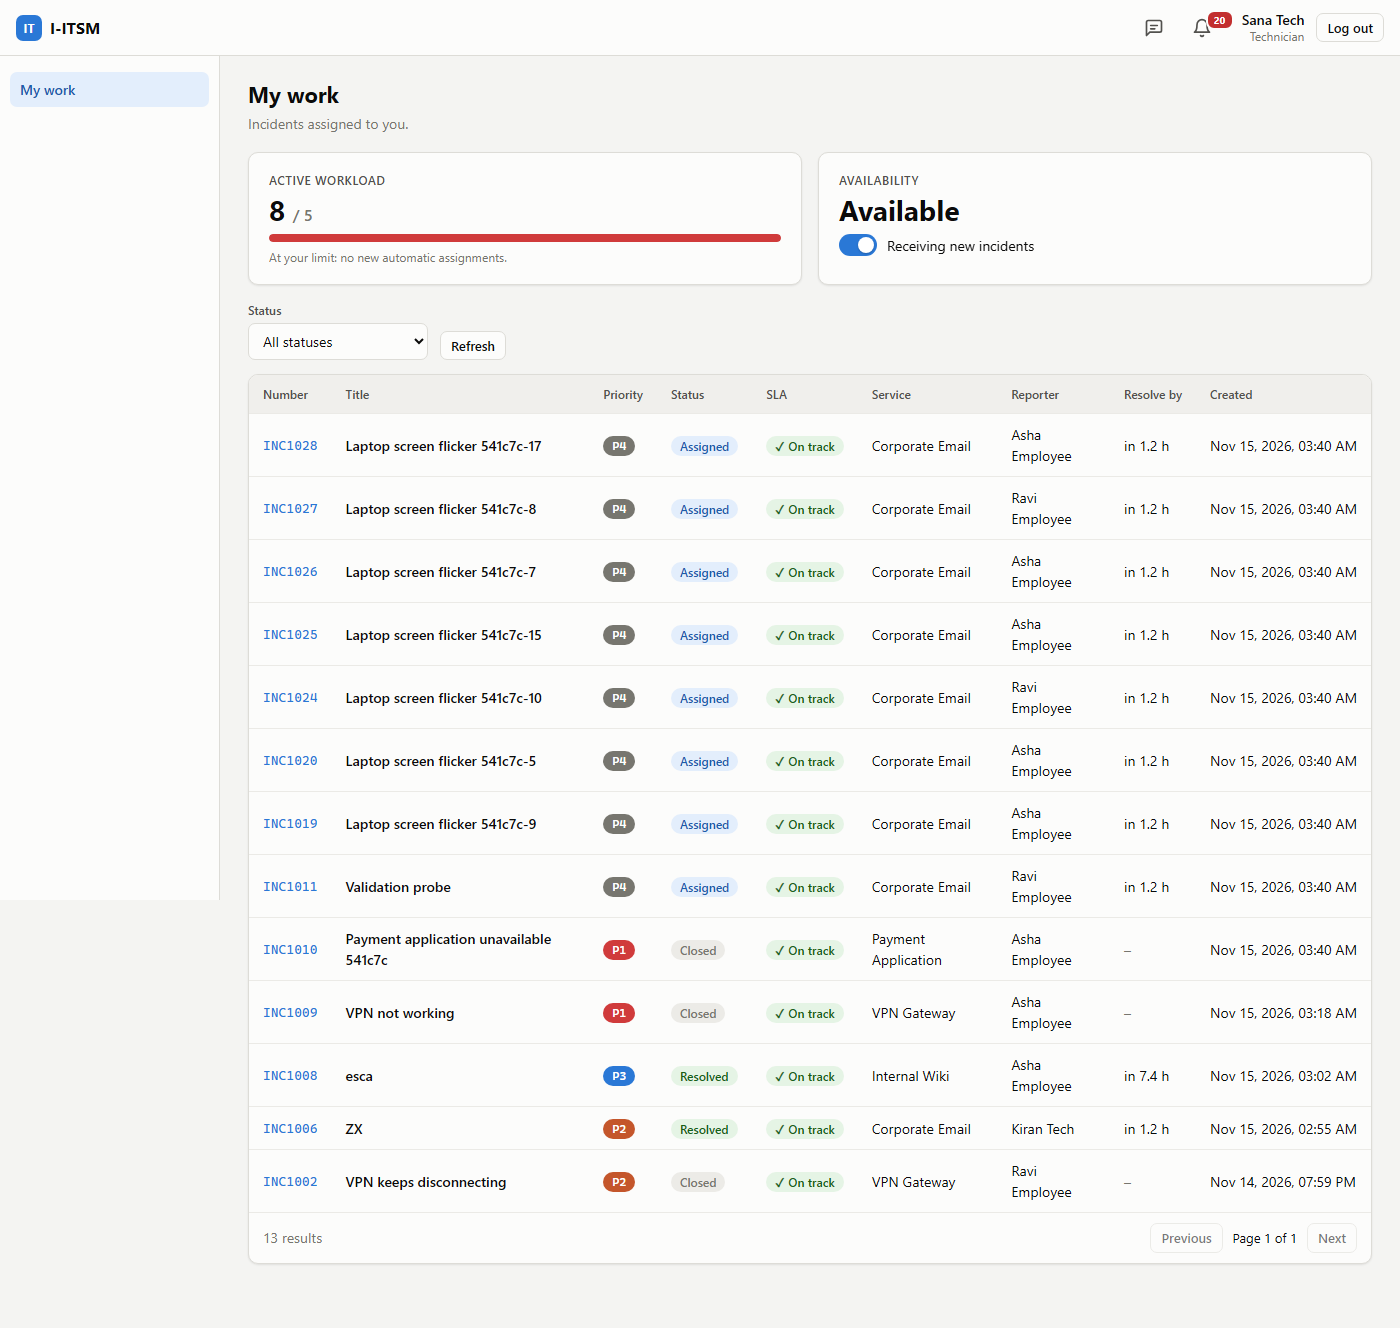
\includegraphics[width=0.8\textwidth]{img/workload-over-limit.png}
\caption{Technician view after 25 concurrent reports: ``Active workload 8 / 5'' (M-01). The RESOLVED rows below still
count down ``Resolve by'' (m-11).}
\label{fig:workload}
\end{figure}

\begin{figure}[h]
\centering
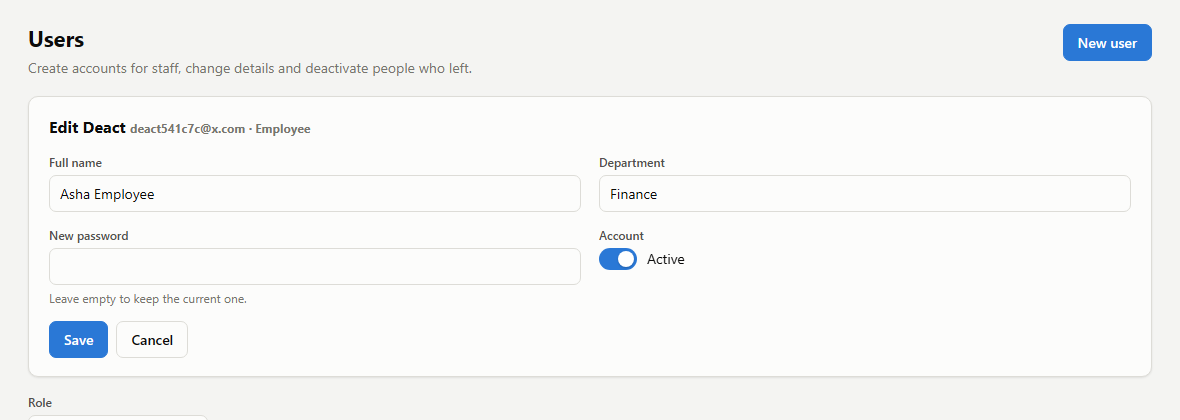
\includegraphics[width=0.92\textwidth]{img/stale-edit.png}
\caption{Users page after clicking \emph{Edit} on ``Asha Employee'' and then on ``Deact'': the heading names Deact, the
fields still hold Asha's data (C-03). Nothing was saved during the audit.}
\label{fig:stale}
\end{figure}

\begin{figure}[h]
\centering
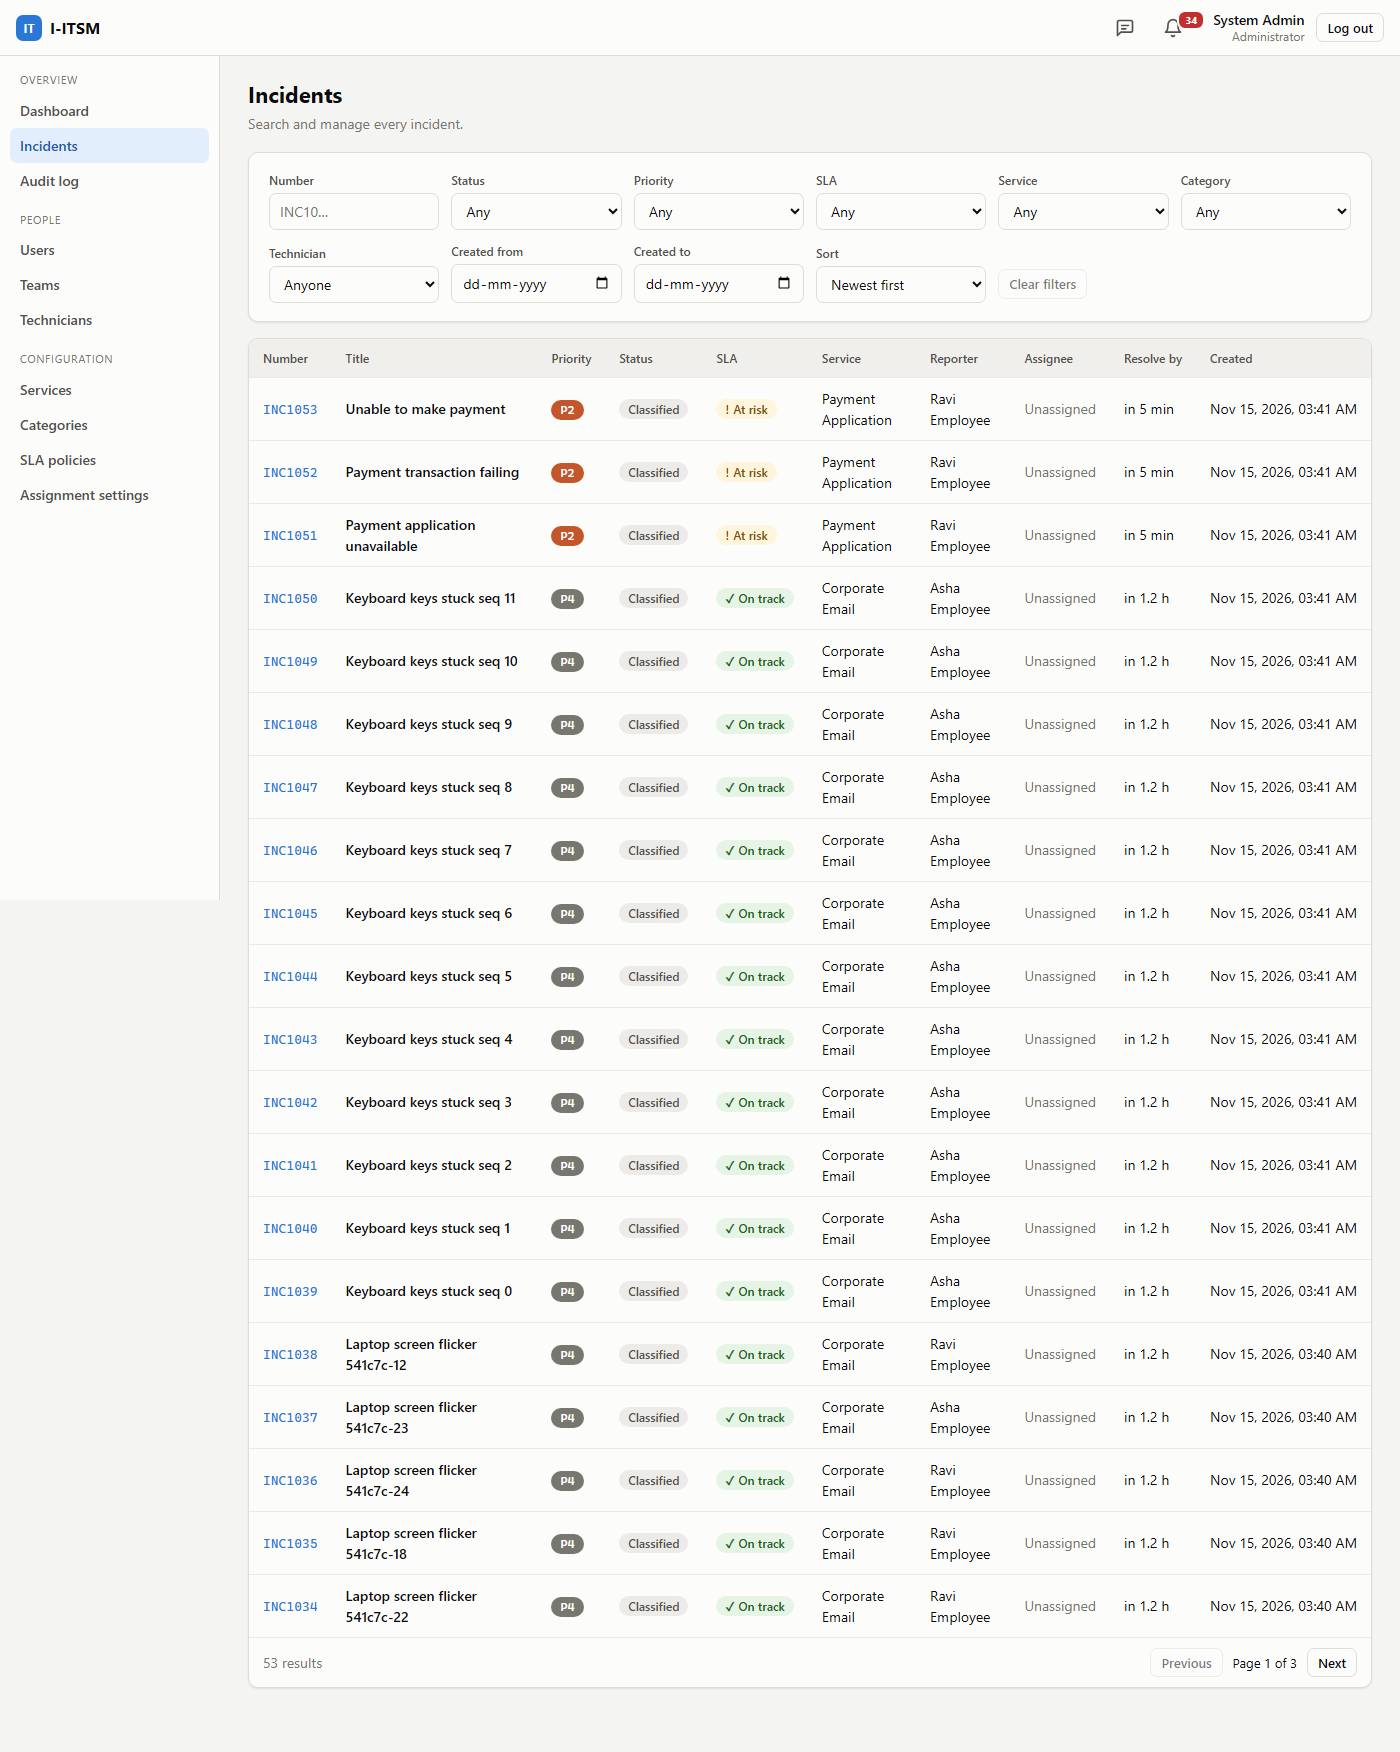
\includegraphics[width=0.92\textwidth,trim=0 1422 0 0,clip]{img/search.png}
\caption{Admin incident search exposes all eight criteria from the specification, including the date range: a requirement that is fully met.}
\end{figure}

\end{document}
